% !TeX spellcheck = da_DK
\section{Følger af apopleksi }
Apopleksi kan forekomme pludseligt, og dermed uden at den ramte kan forberede sig på følgerne. Dette er modsat andre sygdomme,som diabetes, sclerose og KOL, hvor progressionen ofte sker gradvist. Derfor kan der opstå andre psykiske konsekvenser forårsaget af hæmoragisk apopleksi eller iskæmisk apopleksi som f.eks. depression, angst og nedsat funktionsevne, hvilket bl.a. går udover patientens lyst til at komme tilbage til sin normale hverdag \cite{Muus2008} Udover de psykiske konsekvenser giver apopleksi andre følger, som afhænger af, hvilken del af encephalon der rammes og hvor omfangsrig hjerneskaden er. Omfanget afhænger af tiden, hvor en del af encephalon ikke får ilt, størrelse af den eventuelle blødningen og trykket i arterien \cite{Michael-Titus2010}. Følgerne kan både indflydelse på patientens fysiske og mentale tilstand. \\
% ALT DETTE STÅR I INDLEDNINGEN - 75.000 mennesker over 18 år levede i 2011 med følger efter et slagstilfælde \cite{Hjernesagen2015}. Dette tal forventes at være stigende i takt med, at der kommer flere ældre \cite{Sagen2014}. Antallet der dør af hjerneskader har været stagneret de sidste 10 år før 2011, hvor 14 \% døde inden for 30 dage[3]. Det vil derfor kunne forventes, at der er flere, som kommer ud for en hjerneskade og vil have mén herefter, hvilket gør det vigtigt at fokusere på rehabiliteringen for at kunne genoptræne de forskellige kropslige og mentale mangler.


\subsection{Sensoriske og motoriske skader} %Sproglige, sensoriske og motoriske skader
%De sproglige konsekvenser fra apopleksi kaldes afasi. Afasi opleves efter en måned hos 20\% af de apopleksiramte og forekommer oftest ved skade i venstre temporal- og frontallap. De sproglige følger af apopleksi kan skade funktionen til at skrive og tale, men også evnen til at forstå og læse andres tale og skrift. I hvilken grad de sproglige funktioner er berørt kan variere mellem de enkelte patienter, da nogle oplever enkelte formuleringsproblemer, mens andre oplever global afasi. Global afasi gør, at de ramte i nogle tilfælde er helt ude af stand til at kommunikere verbalt eller kun kan fremsige enkelte ord med en vis usikkerhed omkring ordenes betydning.
%De sproglige konsekvenser kan midlertidig bedres med tiden, og flere patienter opnår et kommunikationsniveau, som gør det muligt at begå sig i hverdagen.\cite{Muus2008} \\
Som tidligere nævnt i afsnit \ref{HjerneSenMot} kan apopleksi skade sensoriske såvel som motoriske funktioner. Dette kan bla. opleves som manglende funktion i arme, hænder, ben og fødder. De sensoriske og motoriske konsekvenser er de hyppigst forekommende følger hos apopleksiramte og kan medføre problemer med udførsel af orienterende handlinger. Der kan opstå problemer med forholdet mellem egen krop og objekter omkring sig samt kropdelenes indbyrdes forhold. Desuden kan patienterne have problemer med højre og venstre, og nogle oplever problemer med afstandsbedømmelse. De motoriske følger kan medføre  begrænsninger i bevægelse ift. præcision, generel stivhed, opstart af gang, hurtige og spontane bevægelser samt rystelser. Patienten kan derved have problemer med at gå uden hjælp pga. balanceproblemer eller være uopmærksom på den ene side af kroppen. \cite{Sundhed.dk,DSfA2009}

\subsubsection{Balance}
En motorisk og sensorisk skade kan være balanceproblemer, da både kroppens sanser samt motorik hjælper til opretholdelse af balance. Balancen er vigtig for mennesket, da den opretholder kropsstillingen ved hjælp af ubevidste bevægelser, hvilket også er med til at bevægelse er muligt uden fald. For at opretholde balancen bliver kropsvægten så vidt mulig fordelt omkring kroppens akse og de vægtbærende legemer, herunder fødder i oprejst position og gluteal musklerne i siddende position.\cite{Nichols1997}
Balancen er et komplekst system, da flere forskellige kropssystemer samarbejder om at sende balanceinformation til encephalon, hvor de bearbejdes. Balancen styres f.eks. af proprioceptorer og sansereceptorer i øjne og ører. Samarbejdet mellem receptorerne er illustreret på \figref{flowbalance}. Proprioceptorerne kontrollerer muskler, sener og ledenes position, dvs. proprioceptorerne styrer de ubevidste bevægelser, som hjælper med balancen. \cite{Martini2012} Sansereceptorer opfanger sanseindtryk og videresender informationen til områder i cerebral cortex, cerebellum og til centre i hele truncus encephalicus. Disse områder bearbejder informationen for at konkludere den fysiske position af kroppen og dens lemmer. \cite{Martini2012,Karnath2003} Proprioceptorer og sansereceptorerne, samt hvor de findes, bliver uddybet nærmere i bilag \ref{app-Balance}, hvor der også er en anatomisk forklaring heraf.

\begin{figure}[H]
	\centering
	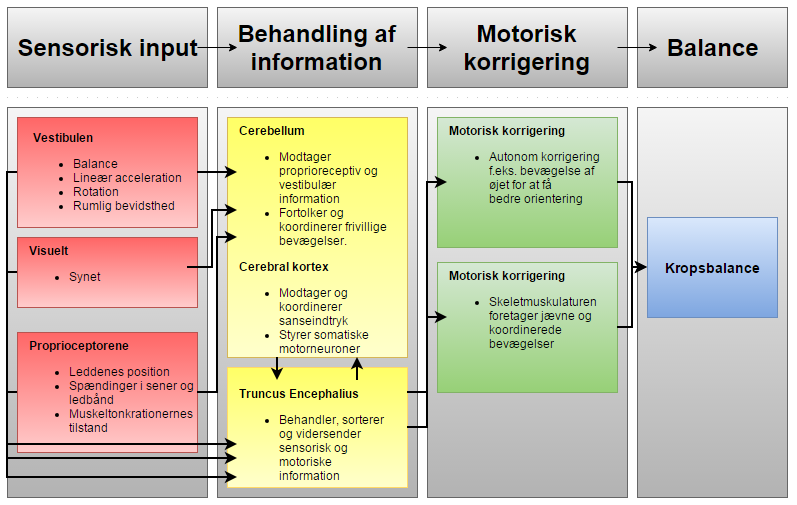
\includegraphics[scale=0.48]{figures/bProblemanalyse/Balance-Flowdiagram.png}
	\caption{På dette flowdiagram ses, hvordan synet, hørelsen og propioreceptorer samarbejder for at opretholde kropsbalancen \cite{watson2015}.}
	\label{flowbalance}
\end{figure}

Apopleksipatienter oplever motoriske og sensoriske skader, da balancen ofte er nedsat eller slet ikke funktionsdygtig.\cite{Karnath2003} Dette skyldes at samarbejdet mellem prorioceptorer og sansereceptorer er svækket og at de behandlede centre i encephalon er skadet. \cite{Martini2012}
Apopleksipatienter kan opleve problemer med balancen i den transversale retning i det frontale plan. Patienterne kan hænge mod deres syge side uden de er opmærksomme på det, hvilket besværliggør funktioner i dagligdagen og giver øget risiko for faldulykker.

\begin{figure}[H]
	\centering
	\includegraphics[scale=1]{figures/bProblemanalyse/Puscher.png}
	\caption{På dette billede ses en patient med puscher syndrom, det er tydeligt at se at patienten krop hænger \cite{Karnath2003}.}
	\label{pusher}
\end{figure}


Et eksempel på, hvordan balancen påvirkes, er Pusher Syndrom. Dette er en lidelse, hvor halvsidigt lammede patienter aktivt skubber deres kropsvægt mod den lammede kropsside, hvilket er illustret på \figref{pusher}. Lidelsen kan opstå som følge af både højre- og venstresidig hjerneskade. Patienter med Pusher Syndrom registrerer ikke, at deres krop hænger, hvilket kan være med til at besværliggøre funktioner i dagligdagen og give øget risiko for faldulykker i både stående, gående og siddende stilling. \cite{Karnath2003} 

\subsubsection{Neglekt}
Neglekt er en sensorisk og motorisk skade, hvilket skyldes at sygdommen kan forekomme visuelt og kropsligt eller i kombination.\fxnote{http://gade.psy.ku.dk/bogkap/neglekt.htm - skal IKKE indsættes i kildeliste, da det ikke er en "pålidelig" kilde, men den er god for os at læse.} Der er mange typer af neglekt og flere kan gøres sig gældende på samme tid, hvilket..... Det anslås at i år 2009 var 25 \% af Apopleksipatienter ramt aaf neglekt. \cite{Sundhedsstyrelsen2009}.Der er mange typer af neglekt og flere kan gøre sig gældende samtidlig \fxnote{kilde!!!!!!!}. 
Ved visuel neglekt kan patienten mangle sanseindtryk fra den påvirkede side af kroppen. Patienten er eksempelvis ikke opmærksom på den ene side af teksten, når vedkommende skal læse, selvom synet er normalt. Derudover kan patienten opleve kun at spise fra den ene del af tallerkenen, eftersom encephalon ikke registrerer den anden halvdel. Ved den kropslige neglekt har patienten manglende kropsbevidsthed. Patienten har ofte normal følelse i den syge side af kroppen - indtrykkene bemærkes, men registres ikke i encephalon. Dette kan komme til udtryk idet patienten glemmer at klæde den syge side af kroppen ordentligt på eller kun barbere halvdelen af ansigtet. En alvorlig følge af dette er, at patienten kan udføre ubevidst skade på sig selv, f.eks. ved at støde ind i ting med den syge side eller ikke være opmærksom på, at benene ikke kan bære kropsvægten. Derved kan der på længere sigt forekomme ergonomiske skader andre steder i kroppen. \cite{Sundhed.dk}

Patienter med neglekt er ikke opmærksomme på den ene side af kroppen.
\subsection{Personlige følger}
Dette afsnit er baseret på hjerneskader generelt. Dvs. det ikke er sikkert, at apopleksi er årsagen, men det antages, at de samme udfordringer gør sig gældende hos personer, der får hjerneskader af apopleksi. Derudover skal det noteres, at det ikke er sikkert, at en patient får følger af apopleksi.

Personer der første gang rammes af en hjerneskade, beskriver hjerneskaden som et brud i deres liv, som de skal lære at forholde sig til. Derudover kan det tage tid for patienterne at indse, at de er ramt af en sygdom. Hjerneskaden går ind og influerer den ramtes humør, personlighed, færdigheder, aktiviteter samt sociale relationer. Patienterne er ikke i stand til at udføre de samme opgaver som tidligere, hvilket påvirker deres identitet. Kroppens funktionsændringer gør, at den ramte kommer til at leve et mere inaktivt og hjemmeorienteret liv end før. En yngre patient er mere ramt af denne forandring ift. en ældre patient. Dette kan bla. skyldes vanskeligheden i at opretholde sociale relationer og begå sig i hverdagen. Apopleksiramte kan derudover opleve en kropsspaltning, hvor kroppen opleves som et fremmedobjekt. Et objekt, som kan være svært at styre og ikke gør, som patienten vil. \cite{Sundhedsstyrelsen2010}

Der findes skjulte vanskeligheder for patienter med hjerneskade som f.eks. med hukommelse, læsning, regning. Disse skjulte vanskeligheder har også en indflydelse på patientens selvopfattelse og  kan derved være med til at nedsætte livskvaliteten for den enkelte. \cite{Sundhedsstyrelsen2010} 

\chapter{Kroppens balance}\label{app-Balance}
Apopleksipatienter oplever ofte problemer med balancen, da den ofte er nedsat eller slet ikke funktionsdygtig af forskellige årsager. \cite{Karnath2003} Proprioceptorer og sansereceptorer hjælper kroppen med balancen. Proprioceptorerne kontrollerer muskler, sener og leddenes position, hvorimod sansereceptorer er en bestemt slags celler, som er placeret i ørerne og øjnene. \cite{Martini2012} Disse celler sender balanceinformationer til det centrale nervesystem og encephalon. Sansereceptorerne opfanger indtryk fra sanserne, som omsættes til bestemte signaler, der sendes til områder i cerebral cortex, cerebellum og til centre i hele hjernestammen. Her bearbejdes informationen, hvorefter der konkluderes den korrekte fysiske position af kroppen og dens lemmer. Når encephalon har bearbejdet indtrykkene, udsender den nerveimpulser til skeletmuskulaturen om at foretage jævne og koordinerede bevægelser, hvorved kropsbalancen opretholdes.\cite{Martini2012} Der ses et flowdiagram af samarbejdet imellem proprioceptorer og sansereceptorer i øjne og øret på \figref{flowbalance}.

Øjet opfanger lys og er med til orienteringen af kroppen og dens lemmer. Hårceller i øret registrerer derimod f.eks. hovedets bevægelser vha. tyngdekraften. Selvom et balanceorgan er ude af funktion, er kroppen stadig i stand til at opretholde balancen ved hjælp fra andre balanceorganer. Det er til gengæld vanskeligt for kroppen at opretholde balancen, hvis de behandlende centre i encephalon bliver skadet, som det kan ske ved apopleksipatienter. \cite{Martini2012} \\
\begin{figure}[H]
	\centering
	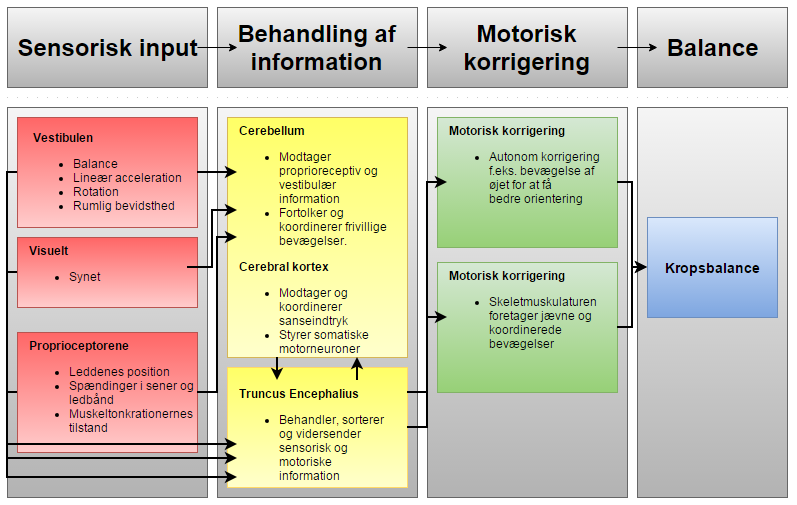
\includegraphics[scale=0.48]{figures/bProblemanalyse/Balance-Flowdiagram.png}
	\caption{På dette flowdiagram ses, hvordan synet, hørelsen og propioreceptorer samarbejder for at opretholde kropsbalancen \cite{watson2015}.}
	\label{flowbalance}
\end{figure}


%\subsection{Identitet}
%En hjerneskadets identitet ændres, da patienten ikke er i stand til at udføre de samme opgaver som tidligere. Derfor bliver den hjerneskadede nødt til at skabe en ny identitet, hvilket for mange kan være svært. Kroppens funktionsændringer gør, at den ramte kommer til at leve et mere inaktivt og hjemmeorienteret liv end før. En yngre patient er mere ramt af denne forandring i forhold til en ældre patient. Apopleksiramte kan derudover opleve en kropsspaltning, hvor kroppen opleves som et fremmet objekt. Et objekt, som kan være svært at styre og ikke gør, som patienten vil.\cite{Sundhedsstyrelsen2010} 

%Der findes skjulte vanskeligheder for patienter med hjerneskade. Disse omfatter vanskelighed med hukommelse, læsning, regning samt andre færdigheder, der ikke er let synlige. Disse skjulte vanskeligheder har også en indflydelse på, hvordan patienten opfatter sig selv og kan være med til at nedsætte livskvaliteten for den enkelte.\cite{Sundhedsstyrelsen2010} 

%\subsection{Patienternes påvirkning}
%Alle de fysiske og mentale ændringer medfører, at det er svært for en hjerneskadet patient at vende tilbage til sit gamle hverdagsliv. Forandringerne gør det svært at udføre almindelige huslige pligter, såsom rengøring og personlig pleje. De ramte oplever det også som en svær oplevelse at vende tilbage på arbejde. Dette skyldes, udover de kropslige og mentale ændringer, også den træthed, der kan opleves. Det er derfor vigtigt at føle sig værdsat på jobbet. Den hjerneskadede patient skal vende tilbage til sine sociale relationer. Dette kan opleves som en meget hård opgave pga. de forandringer, kroppen har gennemgået. Det ses imidlertid, at familierelationerne bliver tættere, mens relationerne til vennerne bliver mindre. Dette er et problem, da gode relationer kan være med til at forbedre rehabiliteringsprocessen og dermed gøre, at den hjerneskadede patient hurtigere kan komme tilbage til et normalt liv.\cite{Sundhedsstyrelsen2010}

%Ud fra  det ovenstående kan det konkluderes, at hjerneskadede patienter, heriblandt apopleksiramte, oplever nedsat livskvalitet pga. deres sygdom. Dette kan også ses ved, at apopleksipatienter har dobbelt så stor selvmordsrate som baggrundsbefolkningen. Derudover nævner 16\% af apopleksi patienter, at deres livskvalitet er dårlig, 46\% syntes den er nogenlunde, mens 38\% synes den er god. Den nedsatte livskvalitet er noget der kan føre til vanskeligheder senere i livet, hvilket selvfølgelig skal forsøges undgået. En forbedret livskvalitet kan skabes ved hurtigere rehabilitering eller forbedret kropslig funktion, som den apopleksiramte patient mistede ved hjerneskaden.\cite{Sundhedsstyrelsen2010}